%%%%%%%%%%%%%%%%%%%%%%%%%%%%%%%%%%%%%%%%%%

\chapter{Commissioning of the nEDM apparatus}\label{chap:nEDM_commissioning_dec2022}

%%%%%%%%%%%%%%%%%%%%%%%%%%%%%%%%%%%%%%%%%%

Engineering run Dec 2022

%%%%%%%%%%%%%%%%%%%%%%%%%%%%%%%%%%%%%%%%%%

\section{Description of experimental setup (2022)}

%%%%%%%%%%%%%%%%%%%%%%%%%%%%%%%%%%%%%%%%%%

Refer user to Chap.~\ref{chap:LANL_nEDM}

Copper guides downstream of switcher

NiP coated electrodes

Experimental control discussed in Chap.~\ref{chap:daq}

%%%%%%%%%%%%%%%%%%%%%%%%%%%%%%%%%%%%%%%%%%

\section{Fill time measurement}

%%%%%%%%%%%%%%%%%%%%%%%%%%%%%%%%%%%%%%%%%%

 \begin{figure}
    \centering
    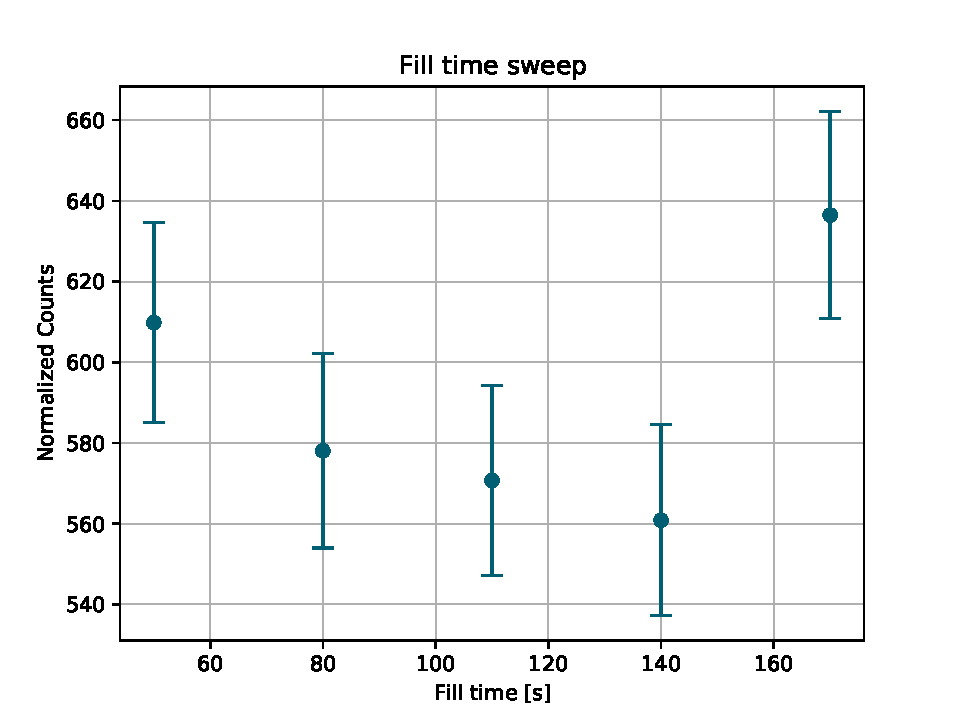
\includegraphics[width=0.6\textwidth]{figures/2022_fill_sweep.pdf}
    \caption
     {Fill-and-dump measurement in the 2022 nEDM apparatus. \qty{100}{s} preload with \qty{30}{s} storage}
    \label{fig:2022_fill_time_sweep}
\end{figure}

Fill time sweep. Normalized to West gate valve. Trying to see if that helps UCN counts (it does not)

%%%%%%%%%%%%%%%%%%%%%%%%%%%%%%%%%%%%%%%%%%

\section{Storage measurement}

%%%%%%%%%%%%%%%%%%%%%%%%%%%%%%%%%%%%%%%%%%

\begin{figure}
\centering
%subfigure width gets "multiplied" by includegraphics width
\begin{subfigure}{.5\textwidth} 
  \centering
  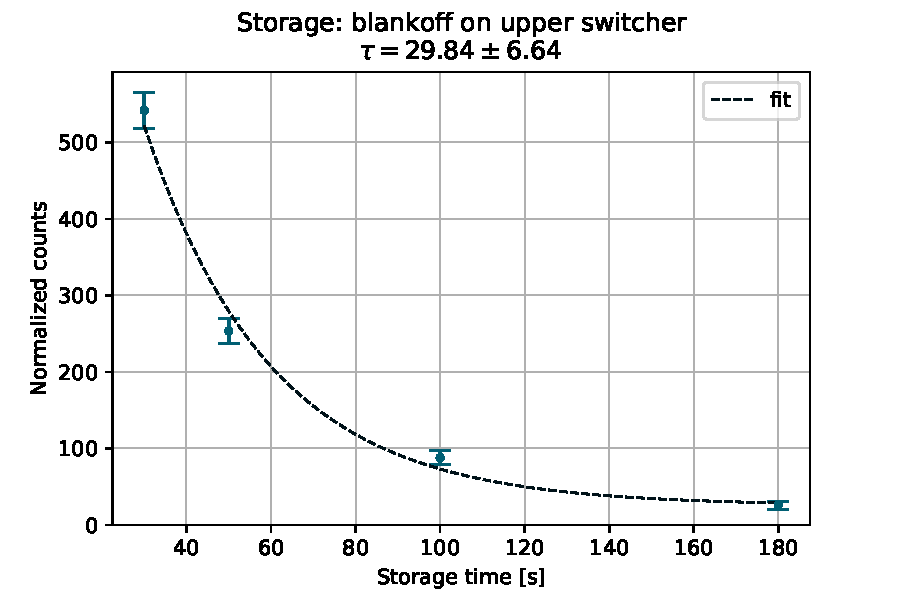
\includegraphics[width=\textwidth]{figures/store_blankoff_fit.pdf}
  \caption{}\label{subfig:2022_storage_blankoff}
\end{subfigure}%DO NOT REMOVE THIS '%'
\begin{subfigure}{.5\textwidth}
  \centering
  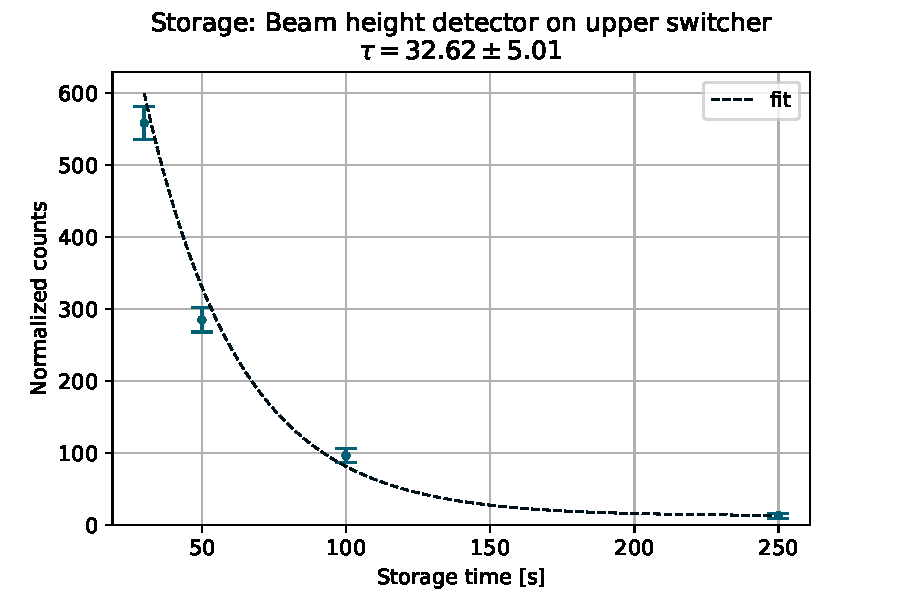
\includegraphics[width=\textwidth]{figures/store_with_beam_height_det_fit.pdf}
  \caption{}\label{subfig:2022_storage_beam_height_det}
\end{subfigure}
\caption
    [UCN storage time measurement in the lower precession cell of the apparatus fit with a single exponential of the form $A \times \exp(-t/\tau) + C$. \textbf{(\subref{subfig:2022_storage_blankoff})} and \textbf{(\subref{subfig:2022_storage_beam_height_det})} differ in terms of where \ucn are directed on the upper switcher.]
    {UCN storage time measurement in the lower precession cell of the apparatus fit with a single exponential of the form $A \times \exp(-t/\tau) + C$. \textbf{(\subref{subfig:2022_storage_blankoff})} and \textbf{(\subref{subfig:2022_storage_beam_height_det})} differ in terms of where \ucn are directed on the upper switcher. \textbf{(\subref{subfig:2022_storage_blankoff})} terminates the upper switcher to a stainless steel blankoff, and \textbf{(\subref{subfig:2022_storage_beam_height_det})} terminates to a beam height \BZnS \ucn detector.}
\label{fig:2022_ucn_storage}
\end{figure}

Load against the closed cell valve to try to see if neutrons get lost there. Then immediately turn the switcher and check guide dump counts are $4350(65)$.

%%%%%%%%%%%%%%%%%%%%%%%%%%%%%%%%%%%%%%%%%%

\section{Single arm spin analyzer benchmark}

%%%%%%%%%%%%%%%%%%%%%%%%%%%%%%%%%%%%%%%%%%


\begin{figure}
\centering
%subfigure width gets "multiplied" by includegraphics width
\begin{subfigure}{.5\textwidth} 
  \centering
  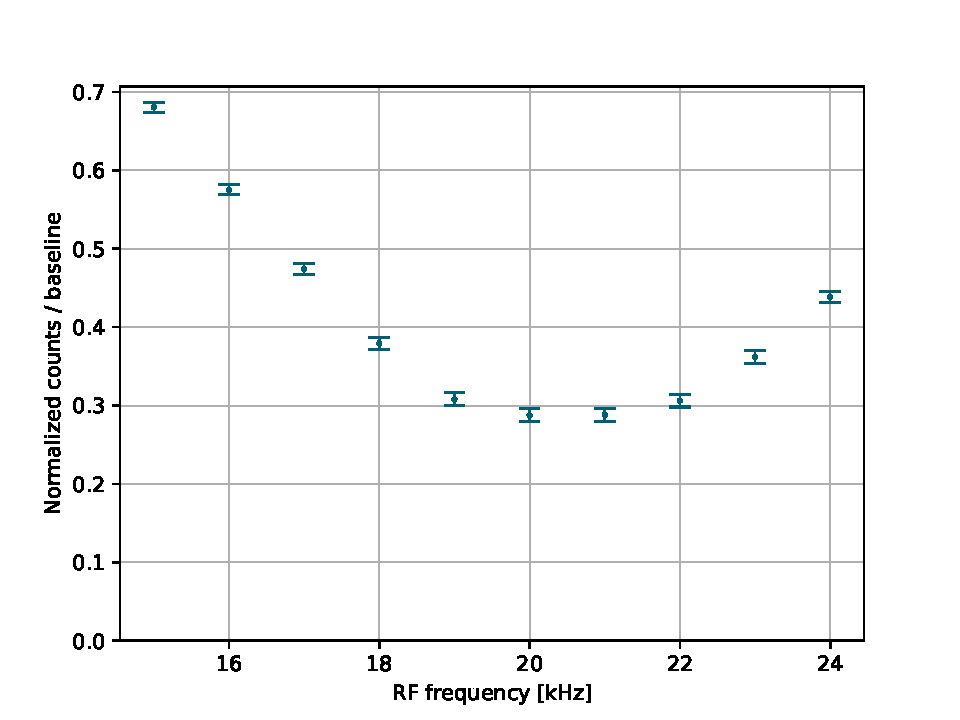
\includegraphics[width=\textwidth]{figures/2022_single_arm_spin_flip_eff.pdf}
  \caption{}\label{subfig:2022_single_arm_eff}
\end{subfigure}%DO NOT REMOVE THIS '%'
\begin{subfigure}{.5\textwidth}
  \centering
  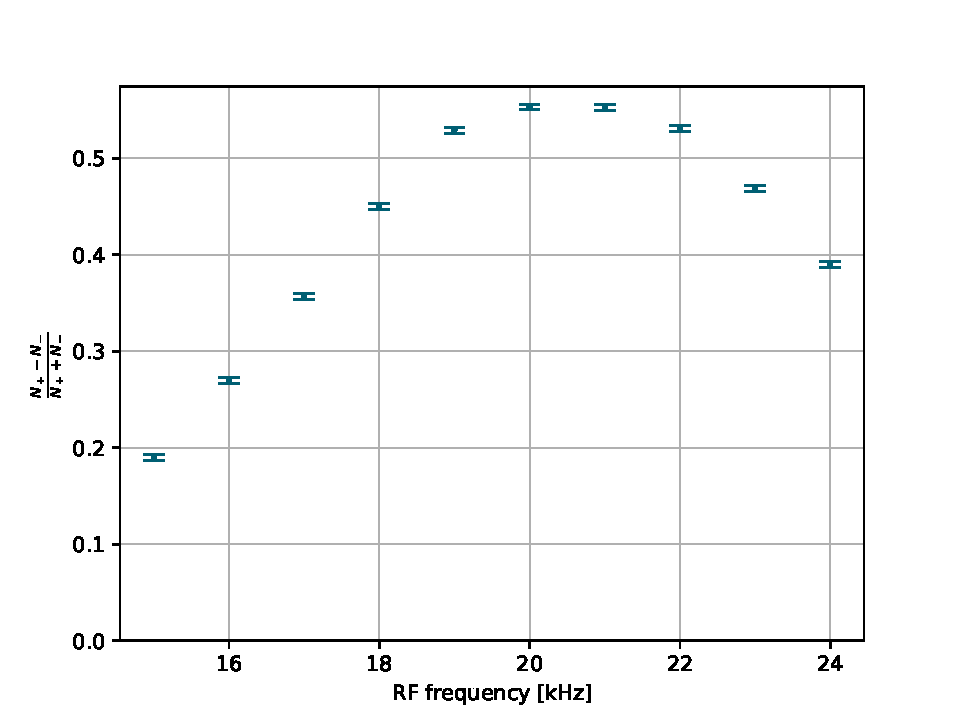
\includegraphics[width=\textwidth]{figures/2022_single_arm_spin_flip_asymmetry.pdf}
  \caption{}\label{subfig:2022_single_arm_asym}
\end{subfigure}
\caption
    {\textbf{(\subref{subfig:2022_single_arm_eff})} Single arm spin flipper efficiency as a function of the RF frequency measured on the North beamline in 2022. The count rate on the y-axis is normalized to the West Gate valve monitor, then divided by the baseline count rate with the spin flipper off. For $\text{Amp}=\qty{10}{Vpp}$, the minimum at \qty{20}{kHz} is 0.28. \textbf{(\subref{subfig:2022_single_arm_asym})} The same data replotted in terms of asymmetry}
\label{fig:2022_single_arm_asymmetry}
\end{figure}

Tuning spin flipper (see Fig.~) in flow through mode. Note the contrast and asymmetry

Comparison of various configurations of holding field coils of single arm vs polarizer in vs out to see how many UCN we are missing. Same procedure each time, with a \qty{100}{s} preload against the NGV, before opening and flowing directly through the lower switcher to spin analyzer. Upper switcher set to beam height detector. Normalized the WGV as usual.

Make a table!!

Foil out: \qty{3404(24)}{UCN\per s}. Beam height: \qty{3657(26)}{UCN\per s}

Foil in (holding field coils OFF): \qty{2747(20)}{UCN\per s}. Beam height: \qty{3836(28)}{UCN\per s}

Foil in (holding field coils nominal): \qty{2744(20)}{UCN\per s}. \qty{3825(28)}{UCN\per s}

%%%%%%%%%%%%%%%%%%%%%%%%%%%%%%%%%%%%%%%%%%

\section{Asymmetry measurements}

%%%%%%%%%%%%%%%%%%%%%%%%%%%%%%%%%%%%%%%%%%

%%%%%%%%%%%%%%%%%%%%%%%%%%%%%%%%%%%%%%%%%%

\section{Discussion}

%%%%%%%%%%%%%%%%%%%%%%%%%%%%%%%%%%%%%%%%%%

Refer to simulation. Can be any number of issues. Transport coils into the MSR. Magnetized components that are saturated on the beamline.